\documentclass[tikz, crop, border = {2pt 2pt 2pt 2pt}]{standalone}

\usepackage{concmath-otf}
\usetikzlibrary{calc, angles, quotes, patterns}
\usetikzlibrary{decorations.pathreplacing, calligraphy}

\begin{document}
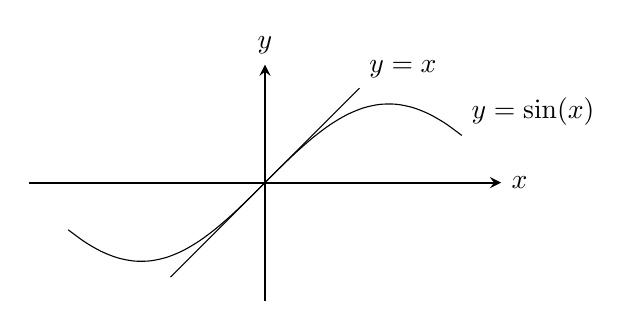
\begin{tikzpicture}
	\draw[-stealth, thick] (-3, 0) -- (3, 0) node[right]{$x$};
	\draw[-stealth, thick] (0, -1.5) -- (0, 1.5) node[above]{$y$};
	
	\draw[domain = -2.5:2.5, smooth] plot (\x, {sin(\x r)});
	\node[above right] at (+2.5, {sin(2.5 r)}){$y = \sin(x)$};
	\draw (-1.2, -1.2) -- (1.2, 1.2) node[above right]{$y = x$};
\end{tikzpicture}
\end{document}
